% Title: Block diagram of Third order noise shaper in Compact Disc Players
% Author: Ramón Jaramillo
\documentclass[tikz,14pt,border=10pt]{standalone}
%%%<
\usepackage{verbatim}
\usepackage{amsmath}
%%%>
\usepackage{textcomp}
\usetikzlibrary{shapes,arrows}
\begin{document}
% Definition of blocks:
\tikzset{%
  block/.style    = {draw, thick, rectangle, minimum height = 3em,
    minimum width = 6em},
  sum/.style      = {draw, circle, node distance = 2cm}, % Adder
  input/.style    = {coordinate}, % Input
  output/.style   = {coordinate} % Output
}
% Defining string as labels of certain blocks.
\newcommand{\suma}{\Large$+$}
\newcommand{\inte}{$\displaystyle \int$}
\newcommand{\derv}{\huge$\frac{d}{dt}$}

\begin{tikzpicture}[auto, thick, node distance=3cm, >=triangle 45]
\draw
	% Drawing the blocks of first filter :
	node at (0,0) []{$y(t) = $}
	node at (0,-1) []{$h_0$}
	node at (6,-1) []{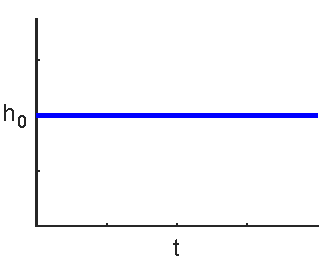
\includegraphics[width=0.28\textwidth]{Plot_h0ex.pdf}}
	node at (0,-2.5) []{$+$}
	node at (0,-4) []{$\sum\limits_{\tau_1=0}^{n_1-1} h_1(\tau_1) u(t-\tau_1)$}
	node at (6,-4) []{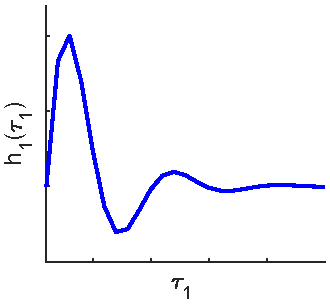
\includegraphics[width=0.28\textwidth]{Plot_h1ex.pdf}}
	node at (0,-5.7) []{$+$}
	node at (0,-7.4) []{$\sum\limits_{\tau_1=0}^{n_2-1} \sum\limits_{\tau_2=0}^{n_2-1}h_2(\tau_1,\tau_2) u(t-\tau_1)u(t-\tau_2)$}
	node at (6,-7.4) []{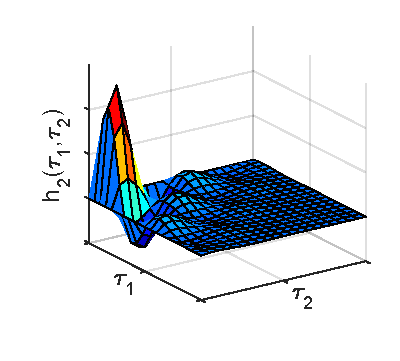
\includegraphics[width=0.35\textwidth]{Surf_h2ex.pdf}}
	node at (0,-9.1) []{$+$}
	node at (0,-10.8) []{$\sum\limits_{\tau_1=0}^{n_3-1} \sum\limits_{\tau_2=0}^{n_3-1} \sum\limits_{\tau_3=0}^{n_3-1} h_2(\tau_1,\tau_2,\tau_3) u(t-\tau_1)u(t-\tau_2)u(t-\tau_3)$}
	node at (6,-11) []{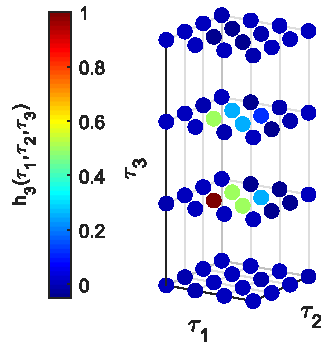
\includegraphics[width=0.28\textwidth]{Scatter3_h3ex.pdf}}
	node at (0,-12.5) []{$+$ higher order terms};
	
%	node at (1,0)[input, name = input2]{}
%	node [block, right of=input1] (sys) {\Huge $\mathcal{S}_0$}
%	node [output, right of=sys](out1) {}
%	node at (5,0)[input, name = input3]{}
%	node at (1,-1.5) [sum](suma1){\suma}
%	node at (5,-1.5) [sum](suma2){\suma}
%	node at (1,-3) [output](out2) {\Large $u$}
%	node at (5,-3) [output](out3) {\Large $y$}
%	node at (-0.5,-1.5)[name=vu]{\Large $v_u$}
%	node at (6.5,-1.5)[name=vy]{\Large $v_y$};
	%node [block, right of=suma1] 
         %node at (6.8,0)[block] (Q1) {\Large $Q_1$}
         %node [block, below of=inte1] (ret1) {\Large$T_1$};
    % Joining blocks. 
    % Commands \draw with options like [->] must be written individually
%	\draw[->](input1) -- node {\Large $u_0$}(sys);
%	\draw[->](sys) -- node {\Large $y_0$}(out1);
%	\draw[->](input2) -- node {}(suma1);
%	\draw[->](input3) -- node {}(suma2);
%	\draw[->](suma1) -- node {\Large $u$}(out2);
%	\draw[->](suma2) -- node {\Large $y$}(out3);
%	\draw[->](vu) -- node {}(suma1);
%	\draw[->](vy) -- node {}(suma2);
 	%\draw[->](suma1) -- node {} (inte1);
	%\draw[->](inte1) -- node {} (Q1);
	%\draw[->](ret1) -| node[near end]{} (suma1);
\end{tikzpicture}
\end{document}